\documentclass[journal,10pt,twocolumn]{article}
\usepackage{graphicx}
\usepackage[margin=0.5in]{geometry}
\usepackage[cmex10]{amsmath}
\usepackage{array}
\usepackage{booktabs}
\usepackage{mathtools}
\title{\textbf{Conic section Assignment}}
\author{Uday kumar Immadisetty}
\date{November 2022}


\providecommand{\norm}[1]{\left\lVert#1\right\rVert}
\providecommand{\abs}[1]{\left\vert#1\right\vert}
\let\vec\mathbf
\newcommand{\myvec}[1]{\ensuremath{\begin{pmatrix}#1\end{pmatrix}}}
\newcommand{\mydet}[1]{\ensuremath{\begin{vmatrix}#1\end{vmatrix}}}
\providecommand{\brak}[1]{\ensuremath{\left(#1\right)}}
\providecommand{\lbrak}[1]{\ensuremath{\left(#1\right.}}
\providecommand{\rbrak}[1]{\ensuremath{\left.#1\right)}}
\providecommand{\sbrak}[1]{\ensuremath{{}\left[#1\right]}}

\begin{document}

\maketitle
\paragraph{\textit{Problem Statement} - If x=9 is the chord of contact of the hyperbola $x^2-y^2=9$ then the equation of the corresponding pair of tangents is}

\section*{\large Solution}

\begin{figure}[h]
\centering
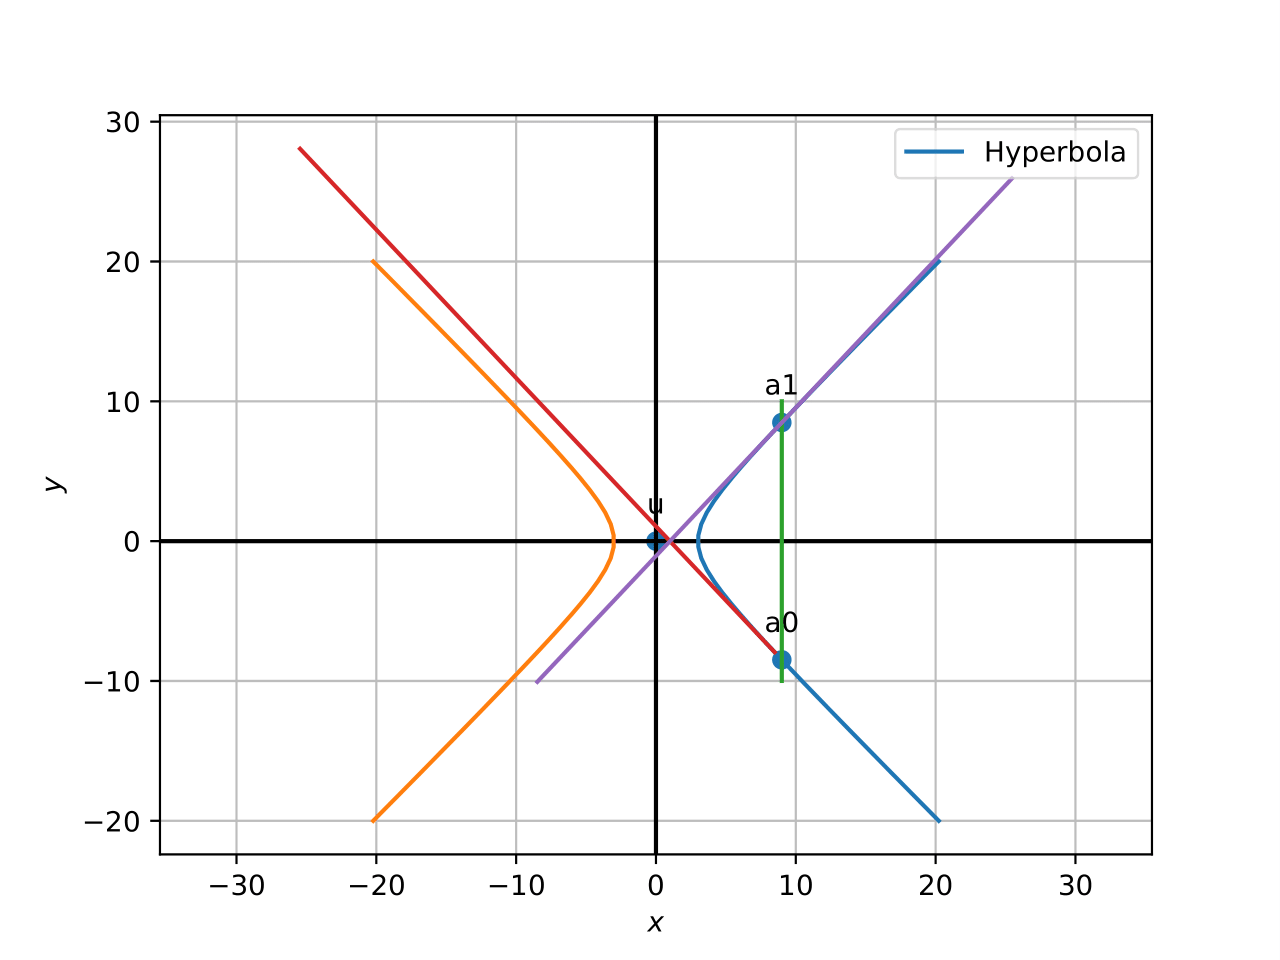
\includegraphics[width=1\columnwidth]{conics1-1.png}

\caption{}
\label{fig:parabola}
\end{figure}

The given equation of hyperbola $x^2-y^2 = 9$ can be written in the general quadratic form as
\begin{align}
    \label{eq:conic_quad_form}
    \vec{x}^{\top}\vec{V}\vec{x}+2\vec{u}^{\top}\vec{x}+f=0
    \end{align}
where
\begin{align}
  \label{eq:V_matrix}
  \vec{V} &= \myvec{1 & 0\\0 & -1},
  \\
  \label{eq:u_vector}
  \vec{u} &= \myvec{0\\0},
  \\
  \label{eq:f_value}
  f &= -9
  %\\
\end{align}



The point of intersection of the lines x=9 and x=4 to the parabola is given by



The points of intersection of the line 
\begin{align}
  L: \quad \vec{x} = \vec{q} + \mu \vec{m} \quad \mu \in \mathbf{R}
\label{eq:conic_tangent}
\end{align}
with the conic section are given by
\begin{align}
\vec{x}_i = \vec{q} + \mu_i \vec{m}
\label{eq:conic_tangent_pts}
\end{align}
%
where
{\tiny
\begin{multline}
\mu_i = \frac{1}
{
\vec{m}^T\vec{V}\vec{m}
}
\lbrak{-\vec{m}^T\brak{\vec{V}\vec{q}+\vec{u}}}
\\
\pm
\rbrak{\sqrt{
\sbrak{
\vec{m}^T\brak{\vec{V}\vec{q}+\vec{u}}
}^2
-
\brak
{
\vec{q}^T\vec{V}\vec{q} + 2\vec{u}^T\vec{q} +f
}
\brak{\vec{m}^T\vec{V}\vec{m}}
}
}
\label{eq:tangent_roots}
\end{multline}
}



From the line x-9=0 the vectors q,m are taken,
\begin{equation}
\vec{q}=\myvec{9\\0}
\end{equation}

\begin{equation}
\vec{m}=\myvec{0\\1}
\end{equation}

by substituting eq(2),(3),(4),(8),(9) in eq(7)
\begin{equation}
\mu_1=-8.48528137
\end{equation}
\begin{equation}
\mu_2=8.48528137
\end{equation}
substituting eq(8),(9),(10) in eq(6) the intersection points on the parabola are
\begin{align}
\vec{a}_0 = \vec{q}+ \mu_1 \vec{m}
\label{eq:conic_tangent_pts}
\end{align}
\begin{align}
\vec{a}_1 = \vec{q}+ \mu_2 \vec{m}
\label{eq:conic_tangent_pts}
\end{align}
Equation of a tangent at a point is 
\begin{align}
({\vec{V}\vec{q}+\vec{u}})^{\top}\vec{x}+\vec{u}^{\top}\vec{q}+f=0
\end{align}

Equation at $a_0$ is 
\begin{align}
t_1 =({\vec{V}\vec{a_0}+\vec{u}})^{\top}\vec{x}+\vec{u}^{\top}\vec{a_0}+f=0
\end{align}

Equation at $a_0$ is 
\begin{align}
t_2 =({\vec{V}\vec{a_1}+\vec{u}})^{\top}\vec{x}+\vec{u}^{\top}\vec{a_1}+f=0
\end{align}
The equation of the corresponding pair of tangents is
\begin{equation}
t = t_1*t_2
\end{equation}
That is 
Equation of pair of tangents is
\begin{align}
t=(({\vec{V}\vec{a_0}+\vec{u}})^{\top}\vec{x}+\vec{u}^{\top}\vec{a_0}+f)(({\vec{V}\vec{a_1}+\vec{u}})^{\top}\vec{x}+\vec{u}^{\top}\vec{a_1}+f)
\end{align}
\section*{\large Construction}

{
\setlength\extrarowheight{5pt}
\begin{tabular}{|l|c|}
    \hline 
    \textbf{Points} & \textbf{intersection points} \\ \hline
  $a_0$ & $\myvec{
   9\\
   -8.48528137
   } $ \\\hline
  $a_1$ & $\myvec{
   9\\
   8.48528137
   } $ \\\hline
      \end{tabular}
}
\end{document}
